% 版权声明 关于本书

\chapter*{版权声明}
由于电子书的种种优势, 我一直对电子书有一种独特的感情, 希望有一天所有的中文教材都能实现电子化. 然而遗憾的是国内的电子教材尚未普及, 这里面可能的原因包括版权保护, 正版销售平台和设备的普及率低等.

而另一方面,即使使用正规平台销售的电子教材,相对于 PDF 文件而言也还有相当的局限性, 包括只能在特定的软件中阅读,注释的种类有限,不支持所有的设备和操作系统,不支持打印等. 

考虑到以上的种种原因, 我最后决定永久提供本书 PDF 的免费下载, 并将捐赠及自觉付款和捐款作为主要的收入方式. 这是一个非常艰巨的决定, 因为本书的写作需要花费大量的时间和精力, 另一方面, 本书的特色之一就是能利用 PDF 文件的普及性, 注释功能, 超链接功能和检索功能等优势.

在未来一段时间内,本书都会仍处于创作阶段(以下称为\bb{非正式版}),内容上有许多不完整.对于非正式版,读者可以免费使用,且在不修改文件的条件下自由拷贝,但也鼓励对本书\bb{捐款}.从本书首个\bb{正式版}起,将要求每位读者在试读累计 3 小时后以自觉付款的形式\bb{购买}本书,否则所持有的任何拷贝都视为盗版.

若发现本书内容有误,请先核对本书最新版核对,再与作者联系.若有任何建议也欢迎联系.最后,若以任何方式引用本书内容或插图,请注明出处并给出链接,在任何出版物上使用本书内容需经过作者同意.

本书的最新版本,作者的联系方式及捐款方式见本书网站 \href{http://littleshi.cn}{\color{blue}littleshi.cn}.

\chapter*{关于本书}

\subsection{1.内容}
% 未完成: 这里要写力学分册! 不是所有内容!

与网络上的百科(例如维基百科)不同的是,《小时物理百科》系列更偏向于教材而不仅仅是一本供专业人士查阅的工具书.本书面向的读者是:1. 具有一定的高中数学物理基础, 但没有上过任何大学数理课程, 想自学大学物理的人. 2. 正在上相关大学物理课程的人( 作为参考书或预习使用). 3. 已学过本书内容, 但需要快速查阅相关内容的人.

本书作为《小时物理百科》系列的第一本(力学分册), 涵盖了物理专业本科生所学的力学课程(通常是第一门专业物理课程)及少许理论力学课程(以下统称为\bb{经典力学})的内容, 以及书中所需的所有超出高考大纲的数学内容(高等数学,线性代数等). 

本书可以帮助读者迅速了解力学的理论框架,配有若干例题,少量习题,不设物理学史等拓展内容, 因此不能代替相关课程的教材.

全书分为两个部分, 数学部分介绍了力学部分涉及的任何超出高中数学的内容, 包括数学拾遗, 一元微积分, 线性代数, 多元微积分与计算物理六章. 与标准的本科高等数学教材(如同济大学的《高等数学》和《线性代数》)相比, 数学部分忽略了许多细节,也忽略了一些物理部分不需要使用的内容.这样,读者可以尽早开始学习物理而无需花费太多时间在数学上.力学部分主要讲解了牛顿的经典力学,包括质点,质点系与刚体,振动与波动,天体运动与中心力场,理论力学五章.

\subsection{2.结构和特点}
与其他教材不同,本书更接近于百科的形式,由许多\bb{词条} 构成. 一个词条从半页到几页不等,可能包括“预备知识”, “结论”, “推导”, “例”, “应用实例”, “拓展阅读” 等不同的组成部分.理论上来说,读者可以直接跳到最感兴的词条,如果“预备知识”里面列出的词条都已经掌握,就可以开始学习该词条\footnote{如果“预备知识”出现在词条开始,则必须先掌握,如果出现在某个小标题下方,则只有阅读该部分时需要掌握},否则就先掌握“预备知识”里面的词条,以此类推.这种学习方法的好处在于无需按照课程的顺序学习, 因此本书在结构上具有很大的优势.  读者甚至可以根据自己的目标词条, 画出一个知识结构图, 这样就可以对知识结构做到一览无余, 用最高的效率攀登目标词条. % 未完成: 这里可以举一个例子: 开普勒三定律.

\begin{figure}[ht]
\centering
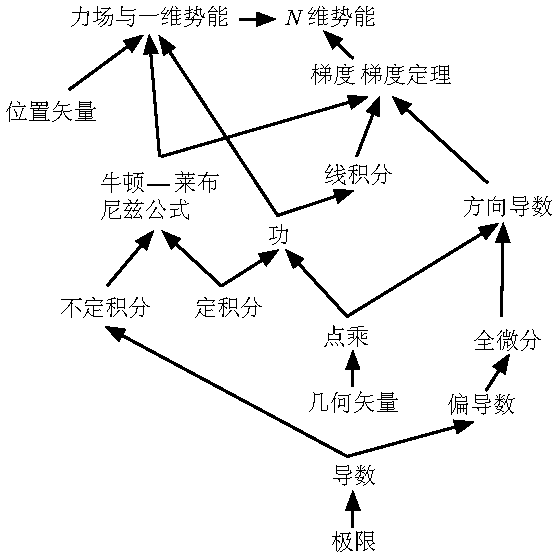
\includegraphics[width=10cm]{./figures/flowchart_example.pdf}
\caption{由“预备知识”画出的知识结构图(目标词条为“力场\ 势能\upref{V}”)}
\end{figure}

需要注意的是,由于本书内容繁多,不同词条的重要性相去甚远,不建议初学者按照词条的排列顺序依次学习,而是应该以每一章节给出的“导航”(第一个词条)为主线来学习,再根据兴趣和需要阅读其余词条.

为了便于书内的跳查,词条之间进行了大量的交叉引用,例如“导数简介\upref{Der}” 右上角中括号中的数字代表被引用词条的页码. 由于每个词条的公式编号都从 1 开始, 引用其他词条中的公式有时会用类似“\autoref{Der_eq2}\upref{Der}” 的格式, 右上角的方括号是公式所在的页码. 在本书的 PDF 电子版中,点击该页码即可自动跳转到对应的页面.在电脑上阅读,推荐使用 Adobe Reader 阅读器,在苹果\textsuperscript{\textregistered} 的 iOS 设备上推荐使用 GoodReader 应用( 两个软件都可以在不同的面板中打开同一本书的不同页码). 在 Adobe Reader 中,使用快捷键组合 “Alt +左箭头” 即可返回跳查前的位置,在移动设备的阅读软件中通常也有相应的返回按钮. 由于本书的电子版是原生 PDF(区别于扫描版), 还具有占用设备存储空间小, 便于分享, 便于查找关键字等种种优势.

\subsection{4.更新}
本书更新速度较快,为保证阅读质量,请及时下载最新版.下载链接见本书网站 \href{http://littleshi.cn}{\color{blue}littleshi.cn}. 如果网页出现故障, 请发邮件到 270174408@qq.com 报错.

%\subsection{5.本书符号约定}
%本书尽量使用物理学教科书中最常使用的符号,列出如下
%用粗体表示矢量,如 $\vec F = m \vec a$,用非粗体表示标量或矢量的模长,如 $\abs{\vec F} = F$.同样用粗体表示矩阵,粗体上方加“$\^$”表示算符
% 未完成


% 物理学专业介绍 % 特别强调理科和工科的区别,介绍物理本科物理一般的学习内容
% 只学习最基础的规律,和模型,知识面广,但不复杂
% 由于太基础,会被认为“没有用”,离应用较远.
% 但物理又是其他理工科的基础
% 物理美在哪里? 更像是“艺术”,从几个最基本的假设出发,由数学推导出许多重要的结果.
% 本书遵循的理念:用尽可能少的公理,和尽可能简单的数学推导出结果,但有尽量保持严谨.
% 数学部分不可能做到像高等数学教材一样严谨,只求易懂且满足本书物理部分的使用.
% 均为本科物理专业教科书的标准内容,自己的内容或者超纲内容会在 “超纲内容” 部分中给出


\chapter*{经典力学及其他物理理论}


%\subsection{牛顿力学}
%牛顿力学主要由牛顿的运动三定律和万有引力定律(也可以拓展到电磁力)构成.
% 未完成,什么是牛顿力学
% 介绍已知的四种作用力

\subsection{物理学理论的可证伪性}

著名的奥地利哲学家波普尔(Popper)对科学的划界是: 一个命题是科学的, 当且仅当它是可证伪的. 如果有人提出一个物理理论,那么既可以尝试用它来计算已有的实验结果,也可以用它来预言一些没有做过的实验结果.如果在实验误差范围内,所有实验与理论计算得到的结果一致,那么就还没有证据表明这个理论是错误的,但也不能说它是绝对正确的.毕竟人们永远也不可能把一个理论的每一种实验,每一套参数都做一遍.然而一旦有一个实验与该理论的计算结果不相符,那么就可以证明这个理论是错误的\footnote{当然首先要考虑是否存在计算错误,实验操作失误,或者存在未考虑到的因素}, 这就是物理学理论的\bb{可证伪性}.

然而可惜的是, 在物理学中目前还没有一个理论可以在任意范围内解释实验或观测结果, 所有的理论(如牛顿力学, 相对论, 量子力学,量子场论) 都只在一定的范围内成立. 我们能做的仅仅是不断创造与实验符合得更精确, 且适用范围更广的理论. 这样一来, 给一个曾经普遍接受的理论打上“错误”的标签似乎有些不妥, 于是我们一般称其为“在适用范围内成立”.


\subsection{物理理论的适用范围\ 经典力学的价值}

经典力学在“宏观低速”的范围内适用.粗略而言,“宏观” 要求物体的质量远大于原子的质量,“低速” 要求物体的速度远小于光速.事实上还有一个条件是 “弱引力场”,例如由于水星离太阳较近,引力场较强,导致其轨道与经典力学的计算出现偏差(轨道进动).所以严格来说,经典力学是一个错误的理论.

若上述中只有“低速” 条件不满足,我们就需要使用狭义相对论,若“弱引力场” 条件不满足,就需要广义相对论(狭义相对论是广义相对论的一部分),若“宏观” 条件不满足,就需要量子力学,若都不满足,那么现在还没有非常完善的理论可以计算(叫做\bb{量子场论,Quantum Field Theory}).

以相对论(狭义和广义的统称)为例,它所适用的范围既包含了经典力学适用的范围,又包含了 “高速” 和 “强引力场”,所以原则上相对论可以完全取代经典力学.由于经典力学在适用的范围内已经得到几百年来大量的实验验证,那么如果相对论是正确的,在经典力学适用的范围内,用相对论计算问题就应该得到同样的结果\footnote{准确来说,二者计算结果的误差需要在实验的测量误差范围内.}.值得注意的是,相对论提出的一些物理概念与经典力学大相径庭.经典的万有引力定律提出任何两个物体之间都存在万有引力,而相对论却指出并不存在引力,而是有质量的物体扭曲了周围的时空,使周围物体的运动方式不同.既然相对论的适用范围更广,那么至少从目前看来相对论提出的原理才是正确的,而经典力学的原理就是错误的. 

既然原理不对,应用范围又相对窄,为什么我们还要先学习经典力学呢? 首先无论在概念上还是数学上,它比相对论简单得多.其次在日常生活或生产中我们接触的绝大部分运动都在经典力学的适用范围内.第三,相对论中同样会出现 “参考系”,“速度”,“能量”,“动量”,等概念,这些概念只有先学习经典力学才会有一个初步的认识,才能继续学习相对论.最后,通过学习经典力学可以了解物理中常见的数学工具,包括一些基础的微积分,矢量分析,线性代数等,这些数学在物理的其他领域更是无处不在.

以上论述同样适用于量子力学与经典力学的关系.量子力学除了经典力学的范围,还包括了 “微观” 范围.总而言之经典力学在现代的物理学中只是一个简单的近似模型,提出的一些概念并不正确,公式也只是一种近似. 一些“民间科学家”时常企图“推翻牛顿定律”, 显然是还不了解这点.

另一方面,即使是相对论和量子力学也并非完美无瑕,通常所说的量子力学是指 “非相对论量子力学”,即同样要求 “低速” 和 “弱引力场”.目前,“相对论量子力学” 的理论还并不完善,是许多理论物理学家努力的方向.




